\documentclass[a4paper]{article}

\usepackage{fullpage} % Package to use full page
\usepackage{parskip} % Package to tweak paragraph skipping
\usepackage{tikz} % Package for drawing
\usepackage{amsmath}
\usepackage{hyperref}
\usepackage{ctex}
\usepackage{amssymb}
\usepackage{amsthm}
\usepackage{indentfirst}
\setlength{\parindent}{2em}
\usepackage{array}
\usepackage{graphicx}
\usepackage{float} 
\usepackage{subfigure}

\renewcommand\thefigure{\thesection.\arabic{figure}}
\makeatletter
\@addtoreset{figure}{section}
\makeatother

\renewcommand\thesubfigure{\thesection.\arabic{figure}(\alph{subfigure})}
\makeatletter
\@addtoreset{figure}{section}
\makeatother

\makeatletter
\renewcommand \theequation {%
	\ifnum \c@section>\z@ \@arabic\c@section.\fi \ifnum \c@subsection>\z@
	\@arabic\c@subsection.\fi\ifnum \c@subsubsection>\z@
	\@arabic\c@subsubsection.\fi\@arabic\c@equation}
\@addtoreset{equation}{section}
\@addtoreset{equation}{subsection}
%\setcounter{section}{-1}
\makeatother
\newtheorem{theorem}{\hspace{2em}定理}[section]
\hypersetup{
	colorlinks=true,
	linkcolor=black
}

\title{高等数值分析}
\author{罗雁天 \\
2018310742}
\date{\today}

\begin{document}

%\maketitle
\newcommand{\HRule}{\rule{\linewidth}{0.5mm}}
\begin{titlepage}
	\begin{center}
		% Upper part of the page
		
\includegraphics[width=0.4\textwidth]{Tsinghua2.png}\\[1cm]
		\textsc{\Large \texttt{高等数值分析}}\\[1cm]
		% Title
		\HRule \\[1cm]
		{\Huge \bfseries 插值程序题}\\[0.4cm]
		\HRule \\[3.5cm]
		% Author and supervisor
		\begin{minipage}{0.4\textwidth}
			\begin{center}
				\Large
				\begin{tabular}{cc}
					\texttt{作者:} & 罗雁天 \\[0.5cm]
					\texttt{学号:} & 2018310742 \\[0.5cm]
					\texttt{日期:} & \today
				\end{tabular}
			\end{center}
		\end{minipage}
		\vfill
	\end{center}
\end{titlepage}

\tableofcontents
\newpage

\section{题目描述}
用多项式函数逼近一般的函数是数值计算的一类基本问题,一来多项式函数形式简单,计算只需有限次加、减、乘、除就可完成,且多项式的导数和原函数还是多项式函数,在不考虑舍入误差时可以在计算机上准确表达和运算;二来,多项式插值来逼近一般的函数还可以用于积分、微分等的运算。

在本次大作业中,我们将利用Newton插值、Lagrange插值、分段线性插值、三次自然样条插值4种插值方式对Runge函数($R(x)=1/(1+25x^2)$)和自定义分段函数$f(x)$(式\ref{eq1})在区间$[-1,1]$上进行插值,并对结果进行分析。

\begin{equation}
\label{eq1}
f(x)=\left\{
\begin{array}{cc}
\sin \pi x & -1\le x< 0, \\
\cos \pi x & 0\le x< 1/2,\\
0 & 1/2\le x \le 1
\end{array}
\right.
\end{equation}

\section{Runge函数的插值分析}
我们首先绘制出Runge函数的真实图像如图\ref{fig:1}所示,其中采样间隔为0.01,一共201个采样点,以此作为我们的标准图像,之后使用4种插值逼近Runge函数的图像与此图像进行对比。

\begin{figure}[!h]
	\centering
	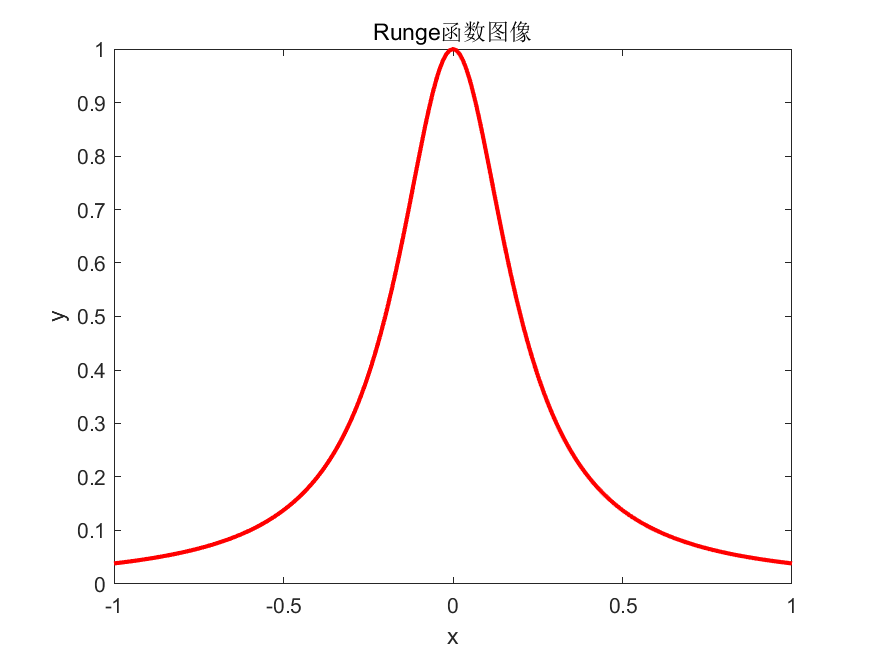
\includegraphics[width=0.8\textwidth]{../code/result/runge}
	\caption{\label{fig:1}Runge函数真实图像}
\end{figure}

\subsection{Newton插值}
使用等距节点$x_i=-1+ih,h=0.1,0\le i\le 20$,对Runge函数进行20次Newton插值。同样选取采样间隔为0.01,一共201个采样点上绘制出20次等距节点Newton插值Runge函数的图像如图\ref{fig:2}所示。可以看出在边界的地方出现了Gibbs现象,与原图像相差极大,由于Newton插值与Lagrange插值等价,因此,我们将此部分的误差分析统一放置到Lagrange插值部分进行分析。从图\ref{fig:2}中我们不能清楚的看出中间部分的插值效果,因此我们将中间局部的插值图像和原图像绘制到一张图上如图\ref{fig:3}所示,从中可以看出,在中间部分插值的结果和原图像是非常相近的。综上,等距节点的Newton插值在非边界部分的逼近效果较好,在边界部分的误差很大,所以等距节点的Newton插值可以求区间内部的值,在边界附近的值误差很大。
\begin{figure}[!h]
	\centering
	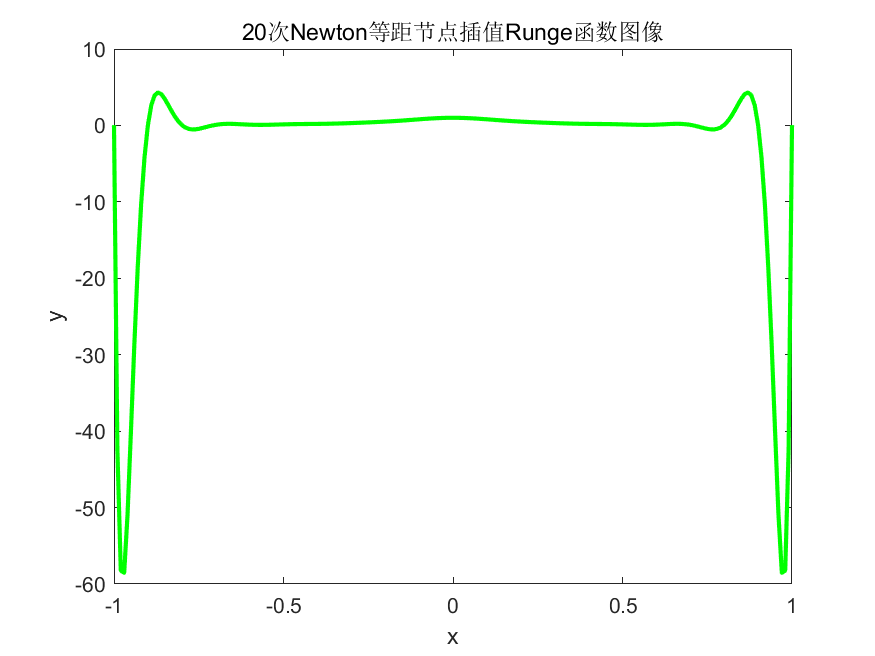
\includegraphics[width=0.85\textwidth]{../code/result/newtonrunge}
	\caption{\label{fig:2}20次Newton等距节点插值Runge函数图像}
\end{figure}

\begin{figure}[!h]
	\centering
	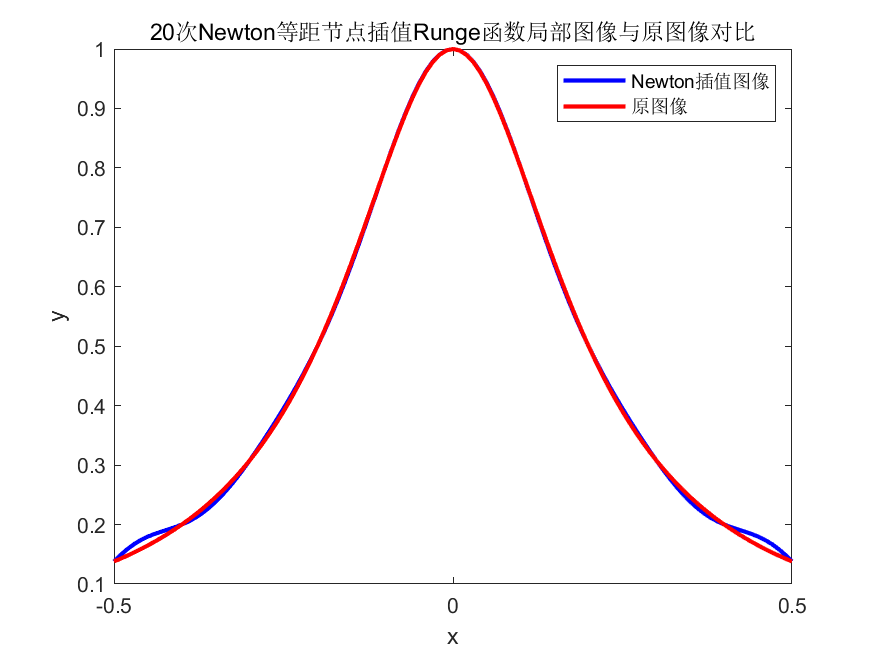
\includegraphics[width=0.85\textwidth]{../code/result/newtonrunge2}
	\caption{\label{fig:3}20次Newton等距节点插值Runge函数局部图像与原图像对比}
\end{figure}

\subsection{Lagrange插值}
为讨论Newton插值的误差,首先我们使用等距节点$x_i=-1+ih,h=0.1,0\le i\le 20$,对Runge函数进行20次Lagrange插值。同样选取采样间隔为0.01,一共201个采样点上绘制出20次等距节点Lagrange插值Runge函数的图像如图\ref{fig:4}所示。为了能够看清区间内部的插值效果,我们绘制出局部图与原图的对比图如图\ref{fig:5}所示,从中可以看出,在中间部分插值的结果和原图像是非常相近的。从图\ref{fig:4}中可以看出在边界的地方出现了与Newton插值一样的Gibbs现象,与原图像相差极大。


\begin{figure}[!h]
	\centering
	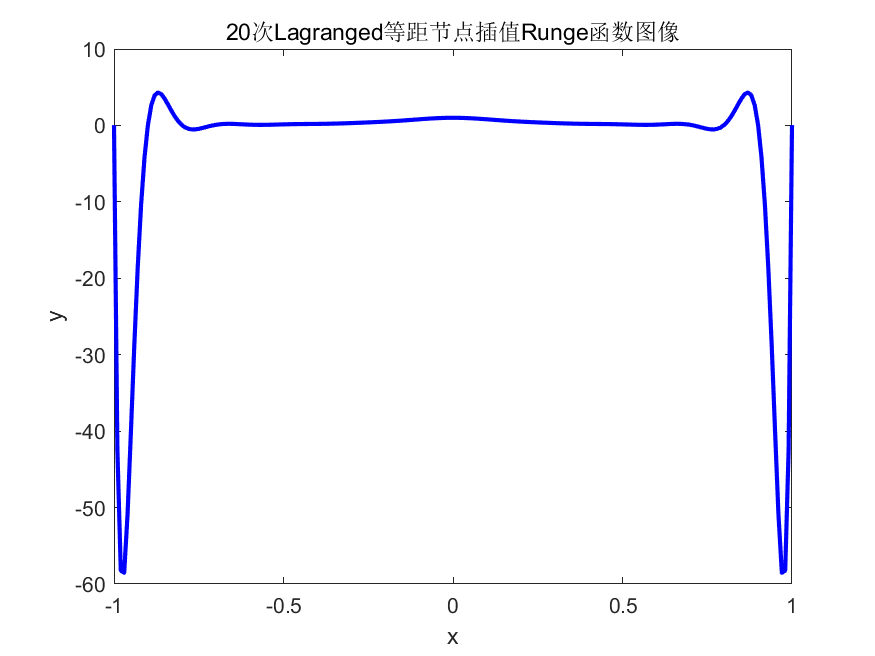
\includegraphics[width=0.85\textwidth]{../code/result/lagrunge}
	\caption{\label{fig:4}20次Lagrange等距节点插值Runge函数图像}
\end{figure}

\begin{figure}[!h]
	\centering
	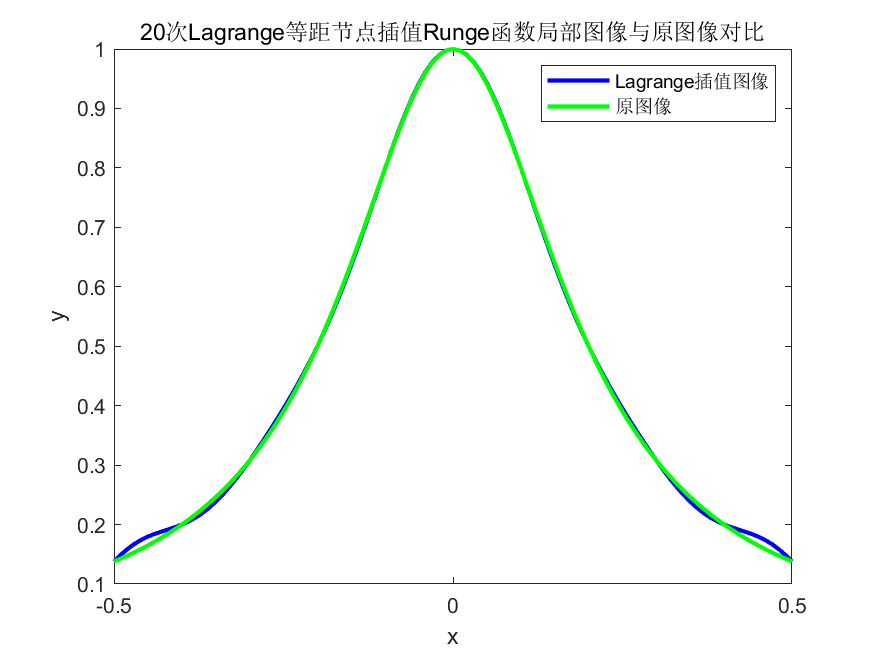
\includegraphics[width=0.85\textwidth]{../code/result/lagrunge2}
	\caption{\label{fig:5}20次Lagrange等距节点插值Runge函数局部图像与原图像对比}
\end{figure}

分析其原因,由于插值函数不可避免存在误差,设$\hat{f_i}=f_i+\epsilon$是扰动后的值,而$\hat{L}_n(x)$是以$\hat{f_0},\hat{f_1},\cdots,\hat{f_n}$为插值数据的多项式,则:

\begin{equation}
f(x)-\hat{L}_n(x)=f(x)-L_n(x)+[L_n(x)-\hat{L}_n(x)]
\end{equation}
而
\begin{equation}
L_n(x)-\hat{L}_n(x)=\sum_{j=0}^{n}\epsilon_jl_j(x)
\end{equation}
假定$n=2m+1,\epsilon_m\ne 0$,其他$\epsilon_j=0$,则
\begin{equation}
|f(x)-L_n(x)|-|f(x)-\hat{L}_n(x)|=\epsilon_ml_m(x)
\end{equation}
由此可以看出,若$l_m(x)$在某些点$x^*$很大,那么$\epsilon_ml_m(x^*)$也变得非常大。这就意味着即使是函数值的微小扰动也将带来插值函数的巨大变化,误差会过分放大。因此我们绘制出在$x=0$点处的节点基函数如图\ref{fig:6}所示,从此图中可以看出,在边界点处的值很大,由此误差被过分放大,出现了等距节点Lagrange插值和Newton插值中的Gibbs现象。 

\begin{figure}[!h]
	\centering
	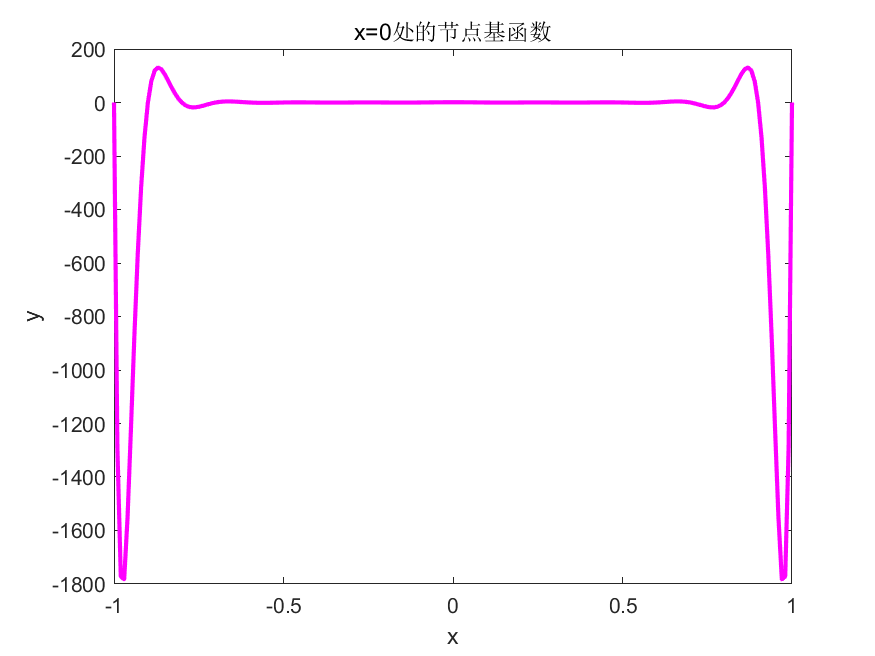
\includegraphics[width=0.85\textwidth]{../code/result/base0}
	\caption{\label{fig:6}x=0处的节点基函数}
\end{figure}

其次我们使用Chebyshev多项式零点进行插值,插值节点为$x_i=cos(\frac{2i+1}{42}\pi)(i=0,1,2,\cdots,20)$.绘制出插值之后的图像如图\ref{fig:7}所示,从图中可以看出,使用Chebyshev多项式的零点作为插值节点插值得到的图像比使用等距节点插值得到的图像效果好很多,在边界点虽然也有波动,但是幅度已经很小了。

\begin{figure}[!h]
	\centering
	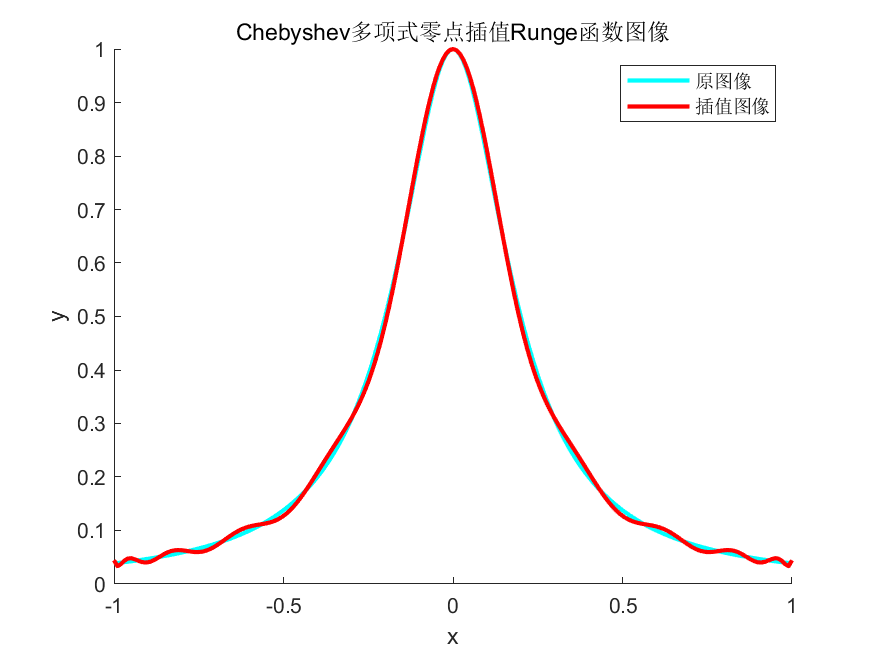
\includegraphics[width=0.85\textwidth]{../code/result/lagche}
	\caption{\label{fig:7}Chebyshev多项式零点Lagrange插值Runge函数图像}
\end{figure}

\subsection{分段线性插值}
使用等距节点$x_i=-1+ih,h=0.1,0\le i\le 20$,对Runge函数进行分段线性插值。同样选取采样间隔为0.01,一共201个采样点上绘制出分段线性插值Runge函数的图像如图\ref{fig:8}所示。从图中可以看出,分段线性插值对原图像的逼近效果是很好的,唯一的缺点便是在插值节点处不光滑,导致图上有毛刺出现,因此在求数值微分的时候使用分段线性插值可能会效果不佳。

\begin{figure}[!h]
	\centering
	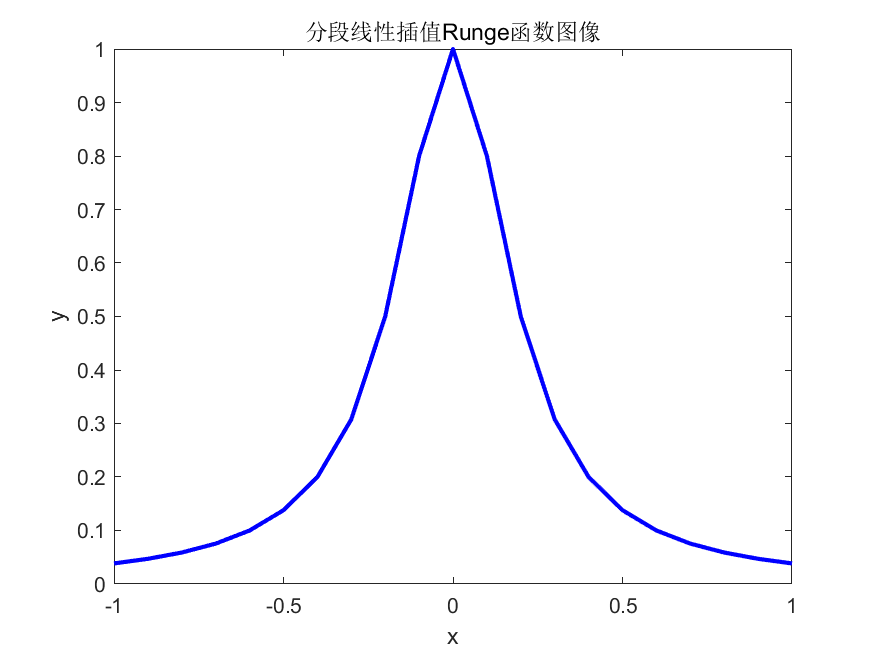
\includegraphics[width=0.85\textwidth]{../code/result/linrunge}
	\caption{\label{fig:8}分段线性插值Runge函数图像}
\end{figure}

\subsection{三次自然样条插值}
使用等距节点$x_i=-1+ih,h=0.1,0\le i\le 20$,对Runge函数进行三次自然样条插值。同样选取采样间隔为0.01,一共201个采样点上绘制出三次自然样条插值Runge函数的图像如图\ref{fig:9}所示。从图中可以看出,三次自然样条插值得到的图像基本与原图像一致,并且足够光滑。结合课上的知识,三次自然样条函数插值满足插值节点的一阶、二阶导数都连续,因此光滑性比分段线性插值要好。

\begin{figure}[!h]
	\centering
	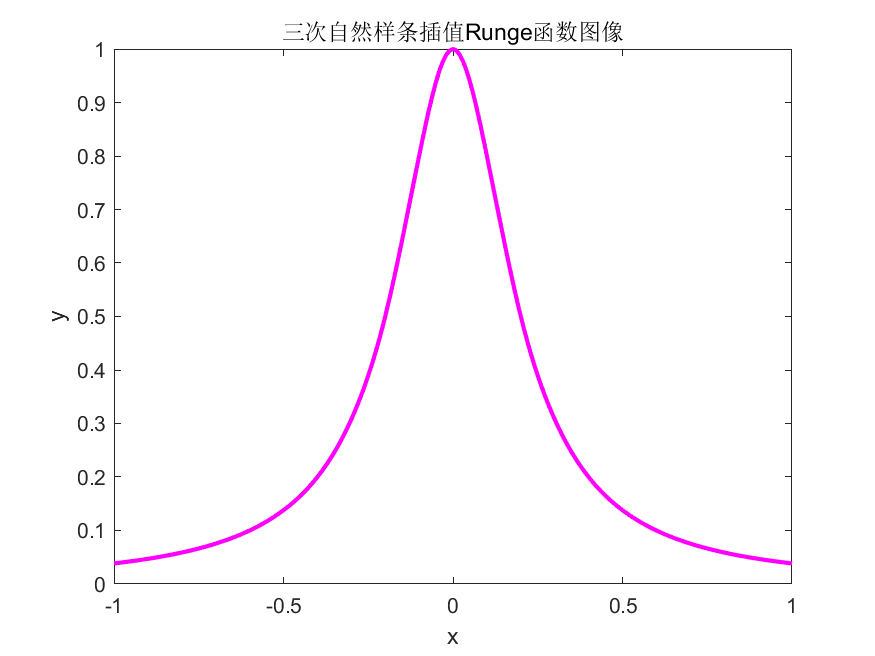
\includegraphics[width=0.85\textwidth]{../code/result/splinerunge}
	\caption{\label{fig:9}三次自然样条插值Runge函数图像}
\end{figure}

\subsection{结论}
综合以上讨论,对于Runge函数而言,采用等距节点的Lagrange(或者Newton)插值在边界点会出现Gibbs现象使得误差极大,不相容,采用Chebyshev多项式零点的Lagrange(或者Newton)插值在边界点虽然会出现波动,但是误差很小,是相容的;采用分段线性插值满足相容性并且误差较之前方法更小,但是其在插值节点不光滑,导数不存在;三次自然样条函数插值,满足相容性,误差最小,并且具有一定的光滑性,在插值节点二阶可导,是对于Runge函数而言最优的插值方式。

\section{不连续函数f(x)的插值分析}
在本节将对不连续函数$f(x)$(式\ref{eq1})利用Newton插值、Lagrange插值、分段线性插值、三次自然样条插值4种插值方式进行分析。

类似的,我们首先做出函数$f(x)$的图像,采样间隔为0.01,共201个采样节点,如图\ref{fig:10}所示。以此作为我们的标准图像,之后使用4种插值逼近Runge函数的图像与此图像进行对比。

\begin{figure}[!h]
	\centering
	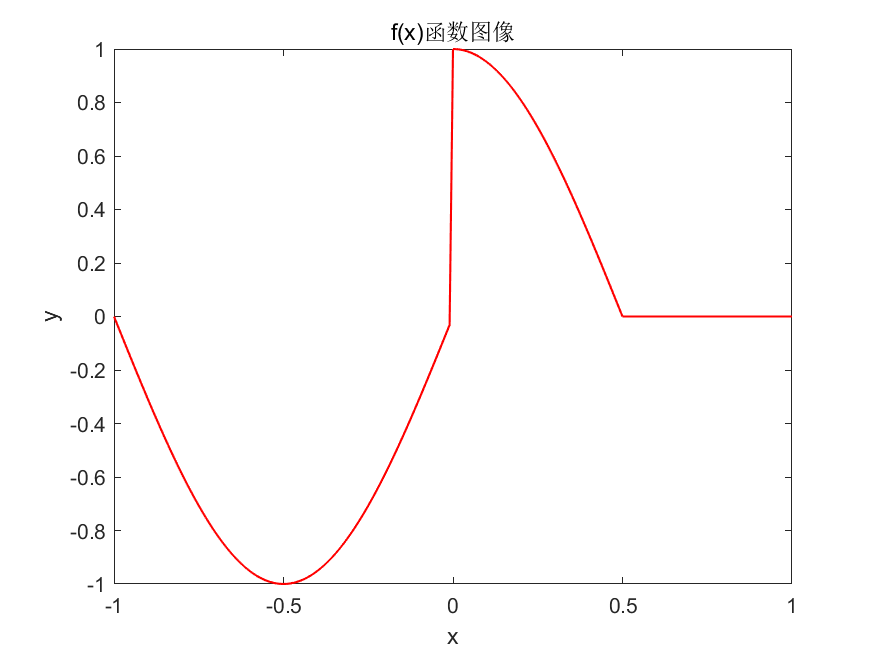
\includegraphics[width=0.85\textwidth]{../code/result/f}
	\caption{\label{fig:10}f(x)函数图像}
\end{figure}

\subsection{Newton插值}
使用等距节点$x_i=-1+ih,h=0.1,0\le i\le 20$,对Runge函数进行20次Newton插值。同样选取采样间隔为0.01,一共201个采样点上绘制出20次等距节点Newton插值Runge函数的图像如图\ref{2fig:1}所示。可以看出在边界的地方出现了Gibbs现象,与原图像相差极大,误差我们已经在之前分析过了,在此不再赘述。

\begin{figure}[!h]
	\centering
	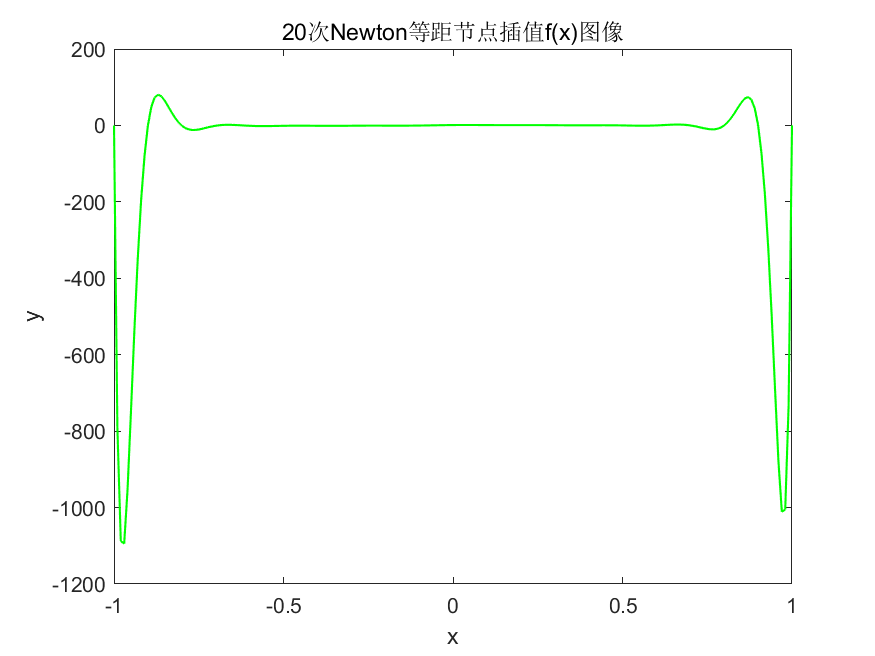
\includegraphics[width=0.85\textwidth]{../code/result/newtonf}
	\caption{\label{2fig:1}f(x)函数图像}
\end{figure}

\subsection{Lagrange插值}
由于等距节点的Lagrange插值结果与Newton插值的结果一致,因此在此不再进行等距节点的Lagrange插值。

我们使用Chebyshev多项式零点进行插值,插值节点为$x_i=cos(\frac{2i+1}{42}\pi)(i=0,1,2,\cdots,20)$.插值图像如图\ref{2fig:2}所示,从中可以看出,插值图像与原图像还是有一定差距的,我们计算采样点的误差,发现在x=0处的相对误差高达30.7676,因此可以发现函数的不连续点对Chebyshev多项式零点Lagrange插值有一定的影响。

\begin{figure}[!h]
	\centering
	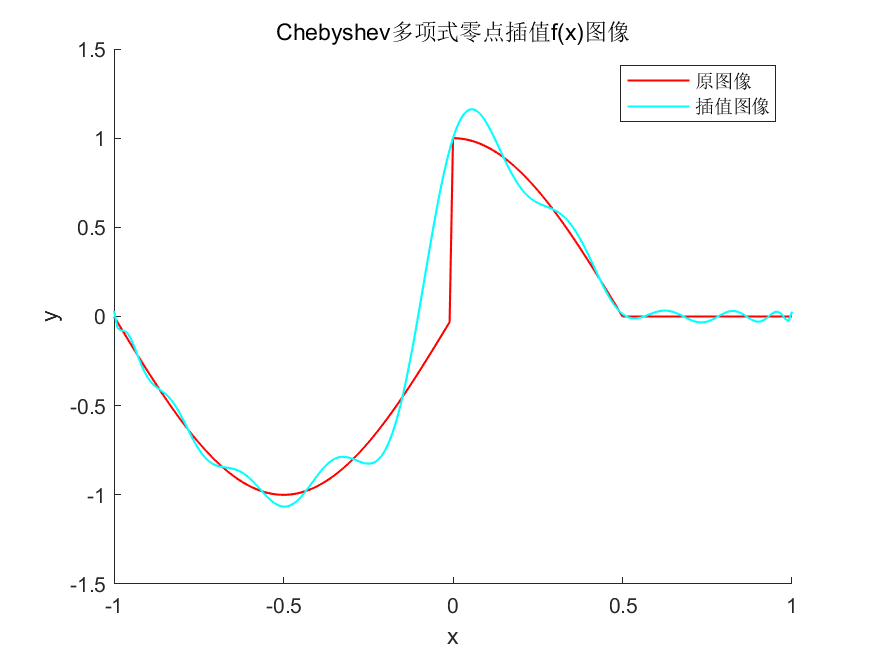
\includegraphics[width=0.85\textwidth]{../code/result/lagchef}
	\caption{\label{2fig:2}Chebyshev多项式零点插值f(x)图像}
\end{figure}

介于此,我们考虑将原始图像的两部分分开进行Chebyshev多项式零点插值,对于左半部分,我们需要使用坐标变换\ref{eq2}将区间放缩到$[-1,1]$之间,对于右半部分,我们需要使用坐标变换\ref{eq3}将区间放缩到$[-1,1]$之间,不妨左侧我们使用10个插值节点,右侧使用11个插值节点,则左侧插值节点为$x_i=\frac{1}{2}(\cos(\frac{2i+1}{20}\pi)-1),i=0,1,\cdots,9$,右侧插值节点为$x_i=\frac{1}{2}(\cos(\frac{2i+1}{22}\pi)+1),i=0,1,\cdots,10$。插值之后的图像与原图像对比如图\ref{2fig:3}所示,由此可以看出,将间断点绕开做分段的Chebyshev多项式零点的Lagrange插值相比于直接做Chebyshev多项式零点的Lagrange插值的效果要好很多,间断点左侧插值效果很好,基本和原图像完全重合,间断点右侧虽然没有与原图像完全重合,但是误差也很小,最大相对误差为0.4526。综上,对于有间断点的函数进行Chebyshev多项式零点插值,可以考虑以间断点进行分段,然后分段插值,效果会好一些。
\begin{equation}
\label{eq2}
x=\frac{t-1}{2},\quad t\in[-1,1] 
\end{equation}
\begin{equation}
\label{eq3}
x=\frac{t+1}{2},\quad t\in[-1,1] 
\end{equation}

\begin{figure}[!h]
	\centering
	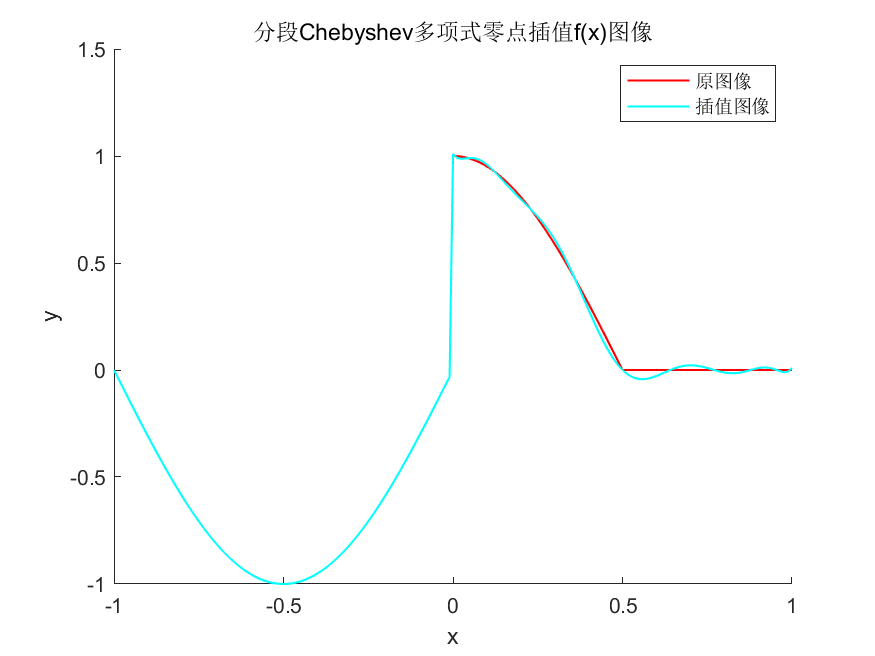
\includegraphics[width=0.85\textwidth]{../code/result/lagchef1}
	\caption{\label{2fig:3}分段Chebyshev多项式零点插值f(x)图像}
\end{figure}

\subsection{分段线性插值}
使用等距节点$x_i=-1+ih,h=0.1,0\le i\le 20$,对分段函数f(x)进行分段线性插值。同样选取采样间隔为0.01,一共201个采样点上绘制出分段线性插值f(x)的图像如图\ref{2fig:4}所示。从图中可以看出,除了间断点附近的逼近效果不好之外,其余点的插值效果都很好。因此,函数间断点的存在也会影响到分段线性插值的一致收敛性,使得在间断点附近出现较大的误差。
\begin{figure}[!h]
	\centering
	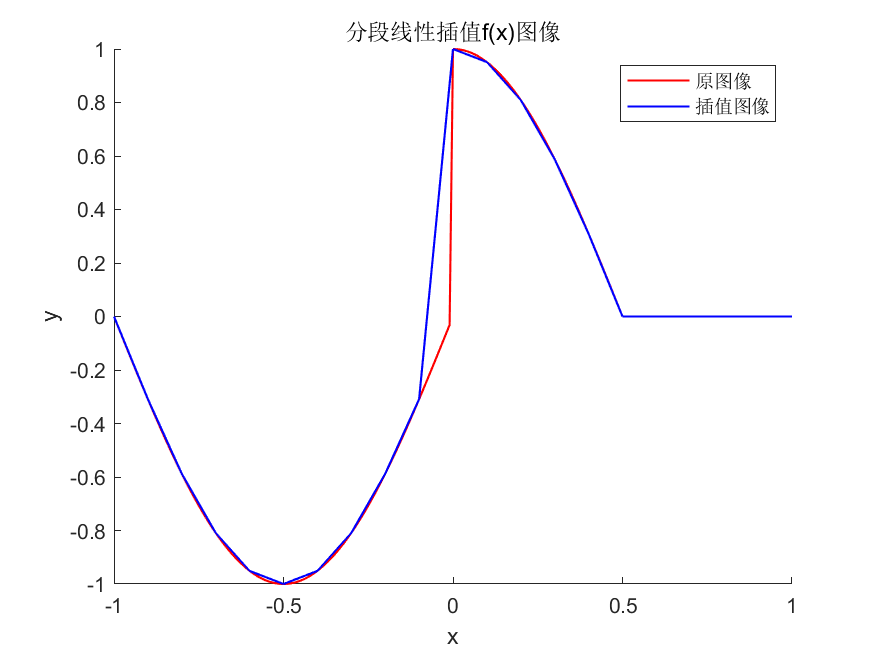
\includegraphics[width=0.85\textwidth]{../code/result/linf}
	\caption{\label{2fig:4}分段线性插值f(x)图像}
\end{figure}

\subsection{三次自然样条插值}
使用等距节点$x_i=-1+ih,h=0.1,0\le i\le 20$,对分段函数f(x)进行三次自然样条插值。同样选取采样间隔为0.01,一共201个采样点上绘制出三次自然样条插值f(x)的图像如图\ref{2fig:5}所示。从图中可以看出,类似于分段线性插值,除了间断点附近的逼近效果不好之外,其余点的插值效果都很好。因此,函数间断点的存在也会影响到分段线性插值的一致收敛性,使得在间断点附近出现较大的误差。

\begin{figure}[!h]
	\centering
	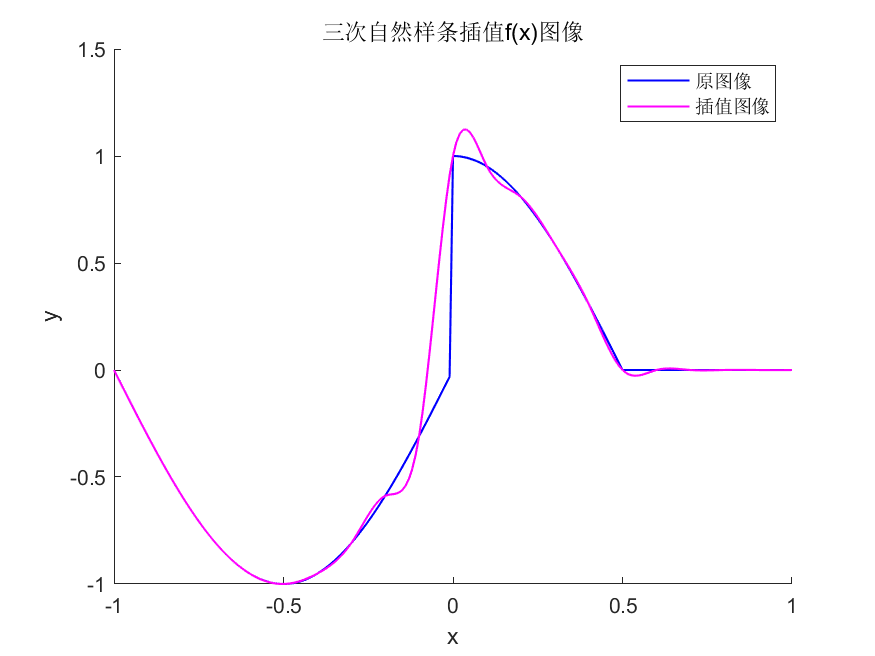
\includegraphics[width=0.85\textwidth]{../code/result/splinef}
	\caption{\label{2fig:5}三次自然样条插值f(x)图像}
\end{figure}

对此,我们将原函数分成左右两部分连续函数,分别采用三次自然样条函数插值,如图\ref{2fig:6}所示,从此图中可以看出,以间断点为界,将原函数分段分别进行三次样条插值的效果很好的减小了间断点附近的误差。

\begin{figure}[!h]
	\centering
	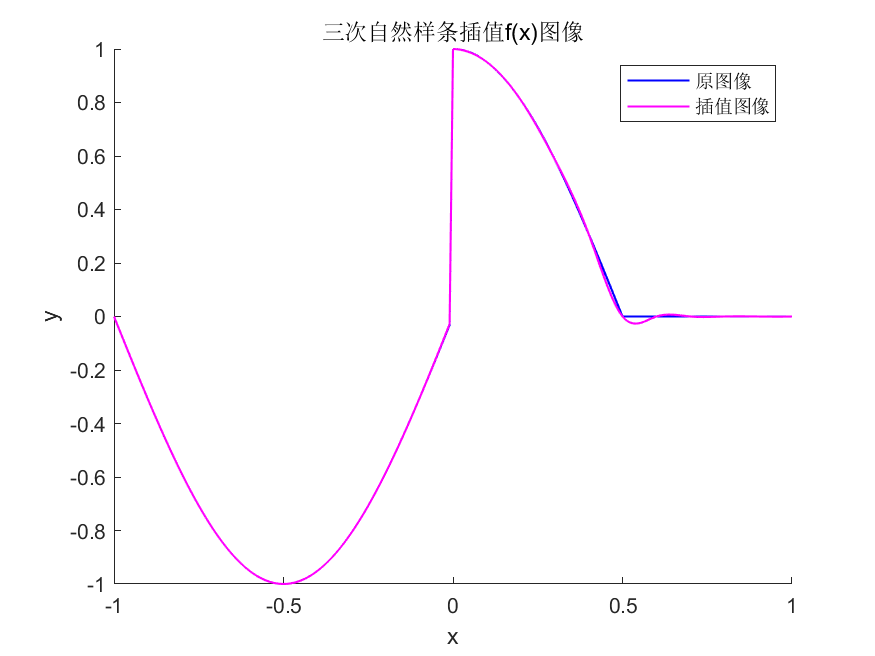
\includegraphics[width=0.85\textwidth]{../code/result/splinef1}
	\caption{\label{2fig:6}以间断点为界,左右两部分分别进行三次自然样条插值f(x)的图像}
\end{figure}

\subsection{结论}
对于有间断点的函数进行插值,等距节点的Lagrange法和Newton法的误差较大,不太适合进行此种函数的插值;直接进行Chebyshev多项式零点的Lagrange插值在间断点附近的误差较大,其他地方误差较小,以间断点为界,分段进行Chebyshev多项式零点的Lagrange插值可以有效地减小间断点附近的误差;分段线性插值和三次自然样条插值插值在距离间断点较远的地方误差很小,在间断点附近误差较大,为了减小间断点附近的误差,可以以间断点为界,分段进行三次自然样条插值来减小误差,但是采用此种方法,会使得在间断点不光滑,打破了三次自然样条插值满足一定光滑性的特点,因此,在误差和光滑性之间还需取舍,使得效果最佳。

\section{实验总结}
本次大作业使用Newton插值、Lagrange插值、分段线性插值、三次自然样条插值4种插值方式对连续函数和有间断点的函数分别进行插值,对比了4种插值方式的特点以及连续函数和有间断点函数插值的区别,复习了巩固了上课讲过的函数插值的知识,对插值有了更加深刻的理解。
\end{document}